%\title{Article HW Template}

\documentclass[12pt]{article}
\usepackage{ucs}
\usepackage[utf8x]{inputenc}
\usepackage[greek,english]{babel}
\newcommand{\en}{\selectlanguage{english}}
\newcommand{\gr}{\selectlanguage{greek}}

\usepackage[paper=a4paper,top=1in, bottom=1in, right=1in, left=.7in]{geometry}


\usepackage{amsthm, amssymb, amsfonts, amsmath}
\usepackage{graphicx}
\usepackage{tikz}
\usetikzlibrary{calc,shapes}
\usepackage{enumitem}
\usepackage{mathtools}
\usepackage{mathrsfs}
\usepackage{tikz-cd}
\usepackage{hyperref, mathabx}
\usepackage{algorithm}
\usepackage{algpseudocode}
\renewcommand{\algorithmicrequire}{\textbf{Input:}}
\renewcommand{\algorithmicensure}{\textbf{Output:}}


\newcommand{\boxitem}[2]{\vspace{.55cm}
	\item[#1]
	\leavevmode
	\strut
	\vadjust{%%
		\noindent
		\raisebox{\dimexpr\dp\strutbox+\ht\strutbox+1ex}[0pt][0pt]{\tikzmark{bl}}}%%
	#2
	
	\leavevmode
	\vadjust{%
		\noindent
		\hspace*{\dimexpr\textwidth+1ex}\tikzmark{br}}%%
	
	\tikz[overlay,remember picture]{\draw[black]
		(bl) rectangle
		(br);}}

\newcommand{\tikzmark}[1]{\tikz[overlay,remember picture] \node (#1) {};}

\newcommand{\R}{\mathbb{R}}
\newcommand{\Q}{\mathbb{Q}}
\newcommand{\Z}{\mathbb{Z}}
\newcommand{\N}{\mathbb{N}}
\newcommand{\p}{\mathbb{P}}
\newcommand{\E}{\mathbb{E}}
\newtheorem*{lemma}{Lemma}
\newtheorem{llemma}{Lemma}
\newtheorem*{theorem}{Theorem}
\newtheorem*{prop}{Proposition}

\begin{document}
	\null\hfill\begin{tabular}[t]{r@{}}
		Nikolas Mavrogeneiadis - 161014\\
		gravitorious \\
		University Of West Attica \\
		Department of Informatics and Computer Engineering\\
		Professor: Panagiotis Rouvelas\\
		\today
	\end{tabular}
	\\
	\centerline{\scshape{Graph Theory-Exercise Set 4}}
	
	\begin{enumerate}[listparindent=1.5em,
		parsep = 0pt]
		
		\gr
		\boxitem{1.}{
			Δείξτε ότι ένας γράφος $G=(V,E)$, είναι συνδεδεμένος αν και μόνο αν για κάθε διαμέριση του $V$ σε δύο μη κενά σύνολα $V_{1}, V_{2}$, υπάρχει ακμή που ενώνει μια κορυφή του $V_{1}$ με μια κορυφή του $V_{2}$.
		}
		Έστω γράφος $G(V,E)$ συνδεδεμένος και έστω μια τυχαία διαμέριση του σε δύο μη κενά σύνολα $V_{1}, V_{2}$. Εστω $x\in V_{1}$ και $y \in V_{2}$. Από υπόθεση υπάρχει $path$ $P$ από το $x$ στο $y$. Έστω $P = \{x=x_{0}, x_{1}, ..., x_{n} = y\}$. Εστω $x_{k}$, $1 \leq k \leq n$, η κορυφή με το μικρότερο $k$ για την οποία ισχύει $x_{k} \in V_{2}$. Επομένως $x_{k-1} \in V_{1}$ και άρα υπάρχει ακμή $e(x_{k-1}, x_{k})$ και επομένως ισχύει το ζητούμενο. \\
		Έστω τώρα ότι για κάθε διαμέριση του $V$ σε δύο μη κενά σύνολα $V_{1}$ και $V_{2}$, υπάρχει ακμή που ενώνει μια κορυφή του $V_{1}$ με μια κορυφή του $V_{2}$. Θα δείξουμε ότι ο $G$ συνδεδεμένος. Έστω ότι δεν είναι. Επιλέγω ως $V_{1}$ να είναι το $set$ που περιέχει μία από τις συνιστώστες του γράφου και $V_{2} = V(G)-V_{1}$. Από υπόθεση υπάρχει μια ακμή από το $V_{1}$ στο $V{2}$, δηλαδή υπάρχει ακμή που ενώνει μια συνιστώσα με μια άλλη. Άτοπο.

		\boxitem{2.}{
			Δείξτε ότι σε κάθε συνδεδεμένο μη πλήρη γράφο $G=(V,E)$ υπάρχουν $u,v,w \in V$ έτσι ώστε $(u,v),(v,w)\in E$ και $(u,w) \notin E$.
		} 
		Δεν είμαι σίγουρος αν είναι σωστή. \\
		Έστω γράφος $G=(V,E)$ με $n=|V|$ συνδεδεμένος και μη πλήρης. Έστω τώρα ότι \\  $\forall u,v,w \in V ((u,v),(v,w)\in E \longrightarrow (u,w) \in E)$. Αν $n=3$, τότε ο γράφος είναι προφανές ότι είναι πληρής. Έστω ότι είναι πλήρης για $k<n$. Έστω μια τυχαία κορυφή $v$ του $G$. Ο γράφος $G-v$ είναι πλήρης από υπόθεση. Έστω ότι προσθέτω τον $v$. Επειδή ο γράφος είναι συνδεδεμένος θα πρέπει να είναι γείτονας με τουλάχιστον μια κορυφή $u$. Η $u$ κορυφή όμως, πριν γίνει γείτονας με την $v$ είχε βαθμό $n-2$. Από υπόθεση θα πρέπει και ο $v$ να συνδεθεί με αυτούς τους $n-2$ κόμβους. Επομένως, όλοι οι κόμβοι έχουν βαθμό $n-1$ και άρα ο $G$ είναι πλήρης. Άτοπο.
		\newpage

		\boxitem{3.}{
			Δείξτε ότι ένας συνδεδεμένος γράφος $G$ είναι ισομορφικός με τον $L(G)$ αν και μόνο αν ο $G$ είναι κυκλικός.
		} 
		Έστω ότι ο $G$ είναι συνδεδεμένος γράφος και ισομορφικός με τον $L(G)$. Έστω ότι $|V(G)| = n$ και $|Ε(G)| = m$. Άρα είναι $|V(L(G))|=m$. Για να ισχύει όμως ο ισομορφισμός, θα πρέπει $|V(G)| = |V(L(G))|$ και άρα $n=m$. Επειδή ο $G$ είναι συνδεδεμένος, μπορούμε να γράψουμε $G = T + e$, όπου $T$ δέντρο και $e$ μια ακμή του $G$. Αν το $T+e$ είναι κυκλικός γράφος τότε το συμπέρασμα ισχύει. Έστω τώρα ότι ο $T+e$ δεν είναι κυκλικός γράφος. Αυτό σημαίνει ότι υπάρχει μια κορυφή $v\in G$ με βαθμό 3. Εύκολα μπορούμε να διαπιστώσουμε  ότι ο $L(G)$ έχει δύο κύκλους ενώ ο $G$ έναν. Άτοπο. 
		\\
		Αντίστροφα, μπορούμε να παρατηρήσουμε ότι αν ο $G$ είναι κυκλικός, τότε και ο $L(G)$ είναι κυκλικός ίδιας τάξης. Επομένως κάθε κορυφή έχει βαθμό τουλάχιστον δύο και άρα μπορώ να βρω έναν ισομορφισμό από το $V(G)$ στο $V(L(G))$.
	
		\boxitem{4.}{
			Έστω $G=(V,E)$, όπου $V$ το σύνολο των μεταθέσεων του $\{1, ..., n\}$, και το $E$ ορίζεται ως εξής: οι κορυφές $(s_{1} s_{2} ... s_{n})$ και $(r_{1} r_{2} ... r_{n})$ συνδέονται με ακμή αν και μόνο υπάρχει $1\leq i < n$ έτσι ώστε $(s_{1} s_{2} ... s_{n}) = (r_{1} r_{2} ... r_{i-1} r_{i+1} r_{i} r_{i+2} ... r_{n})$ (δηλαδή η μία προκύπτει από την άλλη αντιμεταθέτοντας δύο διαδοχικούς όρους της). Δείξτε ότι ο $G$ είναι συνδεδεμένος. Για παράδειγμα, για $n=3$, ο $G$ είναι ο εξής:
			\begin{figure}[h]
				\centering
				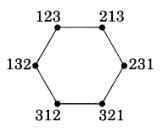
\includegraphics[width=0.20\textwidth]{pic1}
				\caption{}
				\label{fig:mesh1}
			\end{figure}\\ 
		}
		Κάθε κόμβος του γράφου έχει $n!$ κόμβους, όσοι δηλαδή και οι δυνατοί συνδυασμοί. Γνωρίζουμε ότι κάθε μετάθεση μπορεί να προκύψει αντιμεταθέτωντας πολλές φορές δύο γειτονικούς όρους της ακολουθίας. Επομένως μπορούμε από κάθε κορυφή να μεταβούμε σε οποιαδήποτε άλλη κορυφή του γράφου και άρα υπάρχει μονοπάτι μεταξύ κάθε ζευγάρι κόμβων. Άρα ο γράφος έιναι συνδεδεμένος.
		\newpage

		\boxitem{5.}{
			Βρείτε τα τεμάχια των παρακάτω γράφων
			\begin{figure}[h]
				\centering
				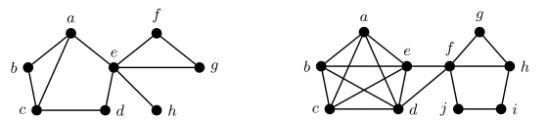
\includegraphics[width=0.50\textwidth]{pic2}
				\caption{}
				\label{fig:mesh1}
			\end{figure}\\ 
		}

		Για τον αριστερά τα τεμάχια είναι: 1)$(a,b,c,d,e)$ και 2)$(e, h)$ και 3) $(f,g,e)$. Για τον δεξιά: είναι: 1)$(a,b,c,d,e,f)$ και 2)$(f,g,h,i,j)$.
		


		\boxitem{6.}{
			Δείξτε ότι δύο διαφορετικά τεμάχια ενός γράφου μπορούν να έχουν το πολύ μία κοινή κορυφή.
		} 
		Έστω δύο τεμάχια $B_{1}$ και $B_{2}$ και ότι έχουν παραπάνω από μια κορυφή κοινή. Ας υποθέσουμε ότι έχουν δύο κοινές κορυφές, $u$ και $v$. Έστω τα μονοπάτια $P_{1}$ και $P_{2}$ από το $u$ στο $v$ του $B_{1}$ και $B_{2}$ αντίστοιχα. Επειδή δύο τεμάχια δεν γίνεται να μοιράζονται μια κοινή ακμή, το ίδιο ισχύει και για τα $P_{1}$ και $P_{2}$. Αυτό όμως σημαίνει ότι μπορώ να δημιουργήσω κύκλο μέ τα $P_{1}$ και $P_{2}$ (παρόμοια θα ίσχυε αν είχαμε παραπάνω από δύο κοινές κορυφές) και άρα υπάρχει κύκλος που περιλαμβάνει και ακμή του $B_{1}$ και του $B_{2}$. Οι ακμές αυτές θα έπρεπε να είναι στο ίδιο τεμάχιο. Άτοπο.

		

	\end{enumerate}
\end{document}
